% !Mode::"UTF-8"
\documentclass[12pt]{article}

% 页面设置
\usepackage{geometry}
\geometry{left=2.5cm, right=2.5cm, top=2.5cm, bottom=2.5cm}  % 设置页边距
\usepackage{graphicx}  % 引用图片
\usepackage{ctex}
\usepackage{fontspec}
\usepackage{setspace}

% 字体设置
\setmainfont{Times New Roman}
\setCJKmainfont{SimSun}
\setCJKsansfont{SimHei}

% 表格设置
\usepackage{makecell}
\newcommand{\addcell}[2][4]{\makecell{\zihao{#1}\textsf{#2}}}
\usepackage{titlesec}
\usepackage{booktabs}
\usepackage{tabularx}

% 设置图注、表注
\usepackage{caption}
\usepackage{bicaption}
\captionsetup{labelsep=quad, font={small, bf}, skip=2pt}
\DeclareCaptionOption{english}[]{
    \renewcommand\figurename{Fig.}
    \renewcommand\tablename{Table}
}
\captionsetup[bi-second]{english}

% 设置页眉
\usepackage{fancyhdr}
\pagestyle{fancy}
\fancypagestyle{preContent}{
    \fancyhead[L]{\zihao{-5} 物理化学实验}
    \fancyhead[C]{\zihao{-5} 实验三\ \ 液体饱和蒸气压的测定}
    \fancyhead[R]{\zihao{-5} 1800011716\ 王崇斌}
}
\pagestyle{preContent}

%	设置首页页眉页脚
\fancypagestyle{plain}{
	\fancyhead[L]{\zihao{-5} 物理化学实验}
	\fancyhead[C]{\zihao{-5} 实验三\ \ 液体饱和蒸气压的测定}
	\fancyhead[R]{\zihao{-5} 1800011716\ 王崇斌}
	\cfoot{}
}

% 设置标题格式
\titleformat*{\section}{\zihao{4}\sffamily}
\titleformat*{\subsection}{\zihao{-4}\sffamily}
\titleformat*{\subsubsection}{\zihao{-4}\sffamily}
\titlespacing*{\section}{0pt}{10pt}{10pt}
\titlespacing*{\subsection}{0pt}{10pt}{5pt}
\titlespacing*{\subsubsection}{0pt}{10pt}{5pt}

% 设置引用格式
\usepackage[super,round,comma,compress]{natbib}
\usepackage{hyperref}  % 使用hyperref包,可以提供文献引用到文件末尾


% 一些相关的包
\usepackage{amsmath}  % 数学公式
\usepackage{amssymb}  % 特殊字符
\usepackage[version=4]{mhchem}  % 用于输入化学式
\usepackage{braket}  % 用于输入Dirac符号
\usepackage{subfigure}  % 多张图片的排版
\usepackage{url}  % 用于引用网址

% 定义常用的命令
\def\d{\mathrm{d}}  % 正体的常用数学常数
\def\e{\mathrm{e}}
\def\i{\mathrm{i}}
\def\dps{\displaystyle}  % 
\newcommand{\mr}[1]{\mathrm{#1}}
\newcommand{\mb}[1]{\mathbf{#1}}
\newcommand{\dv}[2]{\frac{\d{#1}}{\d{#2}}}  % 定义导数、偏导数的简便记号
\newcommand{\pdv}[2]{\frac{\partial{#1}}{\partial{#2}}}
\def\degree{$^{\circ}$}  % 角度
\def\celsius{^{\circ}\mr{C}}  % 摄氏度

%正文
\begin{document}
    % 标题页
    \begin{titlepage}
    	% 页眉
    	\thispagestyle{plain}
        % 图片
        \begin{figure}[h]
            \centering
            \includegraphics{pku.png}
        \end{figure}
        \vspace{24pt}
        % 标题
        \centerline{\zihao{-0} \textsf{物理化学实验报告}}
        \vspace{40pt} % 空行
        \begin{center}
            \begin{tabular}{cp{14.1cm}}
                % 题目
                \addcell[2]{题目:\ } & \addcell[2]{液体饱和蒸气压的测定} \\
                \cline{2-2}
            \end{tabular}
        \end{center}
        \vspace{20pt} % 空行
        \begin{center}
            \doublespacing
            \begin{tabular}{cp{5cm}}
                % 姓名
                \addcell{姓\phantom{空格}名:\ } & \addcell{王崇斌} \\
                \cline{2-2}
                % 学号
                \addcell{学\phantom{空格}号:\ } & \addcell{1800011716}\\
                \cline{2-2}
                % 组别
                \addcell{组\phantom{空格}别:\ } & \addcell{19组} \\
                \cline{2-2}
                % 实验日期
                \addcell{实验日期:\ } & \addcell{2021.09.23}\\
                \cline{2-2}
                % 室温
                \addcell{室\phantom{空格}温:\ } & \addcell{197.26\ K}\\
                \cline{2-2}
                % 大气压强
                \addcell{大气压强:\ } & \addcell{101.18\ kPa}\\
                \cline{2-2}
            \end{tabular}
            \begin{tabular*}{\textwidth}{c}
                \\ % 这是空行
                \\ % 这是空行
                \\ % 这是空行
                \\ % 这是空行
                \hline % 分割线
            \end{tabular*}
        \end{center}
        % 摘要
        \textsf{摘\ \ 要}\ \ 本实验使用静态法测定不同温度下\ce{CCl4}的饱和蒸气压;
		使用动态法测定水在不同压力下的沸点,利用
		Clausius-Clapeyron方程拟合实验结果,得到\ce{CCl4}和水的$\Delta_{vap}H_{m}$分别为
		$31.43 \pm 0.07\,\mr{kJ/mol}$和$41.20 \pm 0.09\,\mr{kJ/mol}$。
		在$p = 101.3\mr{kPa}$下的沸点分别为$76.03\celsius$和$99.73\celsius$;
		摩尔气化熵分别为$90.01\,\mr{J/(mol\,K)}$和$110.50\,\mr{J/(mol\,K)}$,
		对实验和准确值的差异做出了理论解释。
        \\
        \\
        % 关键字
        \textsf{关键词}\ \ Clapeyron方程;饱和蒸汽压;沸点
    \end{titlepage}
	\vbox{}        
    \section{实验部分}
    	\subsection{仪器和试剂}
    	\begin{enumerate}
			\item 试剂:\ce{CCl4},二次去离子水
			\item 仪器:数字式温度-压力测定仪,电加热器,循环水真空泵,冷凝水循环系统,真空缓冲罐,磁力搅拌器等
		\end{enumerate}
    	
		\subsection{实验步骤}
			首先在电脑上安装读取、记录数据的驱动程序,将数字式温度-压力测定仪与电脑连接,调试。
			\subsubsection{静态法测定\ce{CCl4}的饱和蒸汽压}
			按照讲义指导搭建实验装置。首先进行检漏:打开抽气阀门,装置减压至$50\mr{kPa}$左右,关闭抽气阀门,
			如果3min内气压的变化不超过$0.1\mr{kPa}$,说明气密性良好。\\
			开平衡阀通大气,加热至$80\celsius$左右使\ce{CCl4}沸腾,观察到剧烈冒泡;加热过程中,
			c管中的空气逐渐被压入b管排出。关闭加热,观察到沸腾停止,随后b管液面下降,bc两管中液面逐渐接近,
			待c管中无气泡且液面与b管液面水平时,按下“Hold”键,记下压强值和温度值,重复3次,如果度数接近,
			说明空气排尽。\\
			不断降低装置内压力,每次约降低$5\mr{kPa}$,随后测定液面水平时的压强值和温度值,
			直到压力降到约为$50\mr{kPa}$。

			\subsubsection{动态法测定水的饱和蒸汽压}
			在两口烧瓶中盛入约200 mL的去离子水。在各个玻璃接口处涂抹真空脂,按照讲义连接装置,
			使温度探头的前端与水面相切,同前述方法检查气密性。打开冷凝水,
			减压至示数为$50\mr{kPa}$左右,搅拌加热至沸腾,温度和压力稳定后记录数值。
			然后逐渐升高压力(每次约5 kPa),重复记录数据至与大气连通,大气压下的沸点测三次。

	\vbox{}  
	\section{数据与结果}
 		\subsection{静态法测定\ce{CCl4}的饱和蒸汽压}
		装置检漏的数据参见表\ref{static detection}。
		\begin{table}[h]
			\centering
			\zihao{5}
			\bicaption{装置检漏时的气压记录}{pressure document in leak detection}
			\begin{tabular}{ccc}
				\toprule
				时间 & P/kPa & T/$\celsius$ \\
				\midrule
				12:55 & 49.75 & 22.75  \\
				12:57 & 49.81 & 22.74  \\
				12:58 & 49.84 & 22.74  \\
				\bottomrule
			\end{tabular}
			\label{static detection}
		\end{table}
		可以认为装置在实验过程中不漏气。随后通过加热排出c管中的空气,记录b,c两管液面相平时的
		温度和气压,数据参见表\ref{Tb of CCl4 at atm}
		\begin{table}[h]
			\centering
			\zihao{5}
			\bicaption{\ce{CCl4}在大气压下的沸点}{boiling point of \ce{CCl4}}
			\begin{tabular}{cc}
				\toprule
				P/kPa & T/$\celsius$ \\
				\midrule
				 101.02 & 75.95  \\
				 100.98 & 75.98  \\
				 100.99 & 76.02  \\
				 100.98 & 75.97  \\
				\bottomrule
			\end{tabular}
			\label{Tb of CCl4 at atm}
		\end{table}
		从表中看出\ce{CCl4}在大气压下的沸点基本稳定,这说明已经排尽了平衡管ac连接处的空气,可以进行下一步实验。
		在降低体系压力时记录对应的沸点,数据如表\ref{static CCl4}所示。
		\begin{table}[h]
			\centering
			\zihao{5}
			\bicaption{静态法测量\ce{CCl4}饱和蒸气压数据}{vapour pressure of \ce{CCl4} by static method}
			\begin{tabular}{cccc}
				\toprule
				P/kPa & T/$\celsius$ & P/kPa & T/$\celsius$\\
				\midrule
				95.33 & 74.15 & 70.39 & 64.69 \\
				90.48 & 72.44 & 65.50 & 62.47 \\
				85.32 & 70.54 & 60.30 & 60.10 \\
				80.64 & 68.75 & 55.15 & 57.47 \\
				75.38 & 65.70 & 50.08 & 54.74 \\
				\bottomrule
			\end{tabular}
			\label{static CCl4}
		\end{table}
		\par
		首先给出两者之间的关系曲线
		\footnote{
			这里使用了python中scipy.interpolate.interp1d()进行了三次样条插值
		}
		如图\ref{P-T spline of CCl4}。
		\begin{figure}[h]
			\centering
			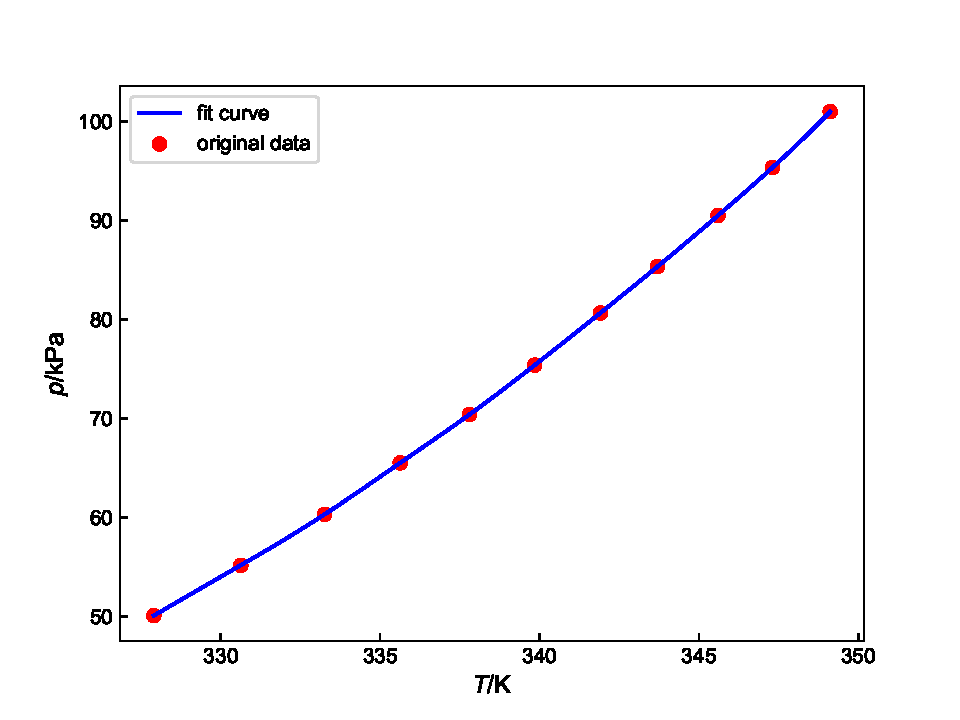
\includegraphics[width=0.6\textwidth]{CCl4_spline.pdf}
			\bicaption{\ce{CCl4}的饱和蒸汽压与温度的关系}{the relation between vapour pressure of \ce{CCl4} and temperature}
			\label{P-T spline of CCl4}
		\end{figure}
		\par 
		考虑使用Clapeyron方程拟合上述实验数据,Clapeyron方程为:
		\begin{equation}
			\dv{p}{T} = \dfrac{\Delta_{vap}H_{m}}{T(V_{g, m} - V_{l, m})}
		\end{equation}
		如果认为在我们实验的区间内气化焓不变(等价于忽略两相之间的热容差),同时忽略掉凝聚相(液相)
		的体积,认为蒸气为理想气体,那么上述方程可以积分为如下形式:
		\begin{equation}
			\ln\left(\dfrac{p}{p^{\circ}}\right) = -\dfrac{A}{T} + B
		\end{equation}
		其中$\Delta_{vap}H_{m} = A * R$,$R$为摩尔气体常数。对实验数据的气压与温度做相应的变换,
		按照上述方程进行线性回归
		\footnote{这其中使用了python的模块scipy.stats.linregress()}
		,结果如图\ref{P-T of CCl4}所示:
		\begin{figure}[h]
			\centering
			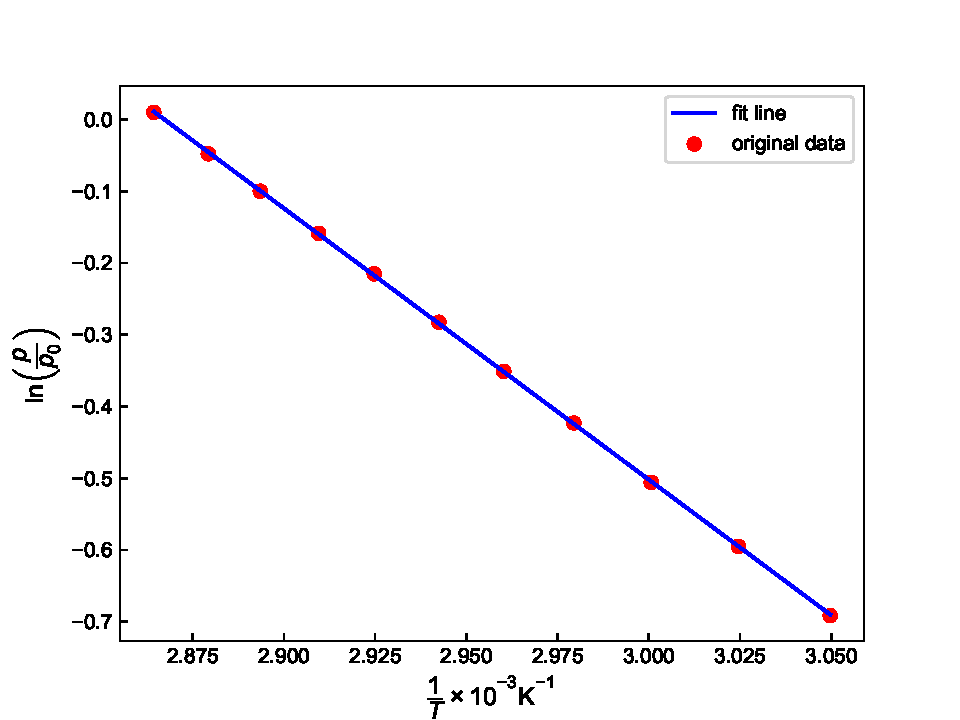
\includegraphics[width=0.6\textwidth]{CCL4.pdf}
			\bicaption{\ce{CCl4}的饱和蒸汽压与温度的关系}{the relation between vapour pressure of \ce{CCl4} and temperature}
			\label{P-T of CCl4}
		\end{figure}
		从图中可以看出很好的线性相关性,同时回归方程为
		\footnote{由于计算蒸发焓并不需要截距的信息,因此这里没有给出截距的不确定度}
		:
		\begin{equation}
			\ln\left(\dfrac{p}{p^{\circ}}\right) = -\dfrac{-3780\pm 8}{T} + 10.84
		\end{equation}
		可以计算出\ce{CCl4}的蒸发焓为$\Delta_{vap}H_{m} = 31.43\pm 0.07\,\mr{kJ/mol}$,
		带入$p = 101.3\mr{kPa}$可以计算出正常沸点为$T_b = 76.0\pm0.2\celsius$。进一步可以计算出
		正常沸点下的摩尔气化熵$\Delta_{vap}S_{m} = 90.0\pm0.2\,\mr{J/(mol\,K)}$,与Trouton规则非常接近。
 		\vbox{}

 		\subsection{动态法测定水的饱和蒸汽压}
		 装置检漏的数据参见表\ref{dynamic detection}。
		\begin{table}[h]
			\centering
			\zihao{5}
			\bicaption{装置检漏时的气压记录}{pressure document in leak detection}
			\begin{tabular}{ccc}
				\toprule
				时间 & P/kPa & T/$\celsius$ \\
				\midrule
				11:48 & 49.28 & 24.69  \\
				11:50 & 49.34 & 24.17  \\
				11:52 & 49.36 & 24.10  \\
				\bottomrule
			\end{tabular}
			\label{dynamic detection}
		\end{table}
		可以认为实验装置不漏气。不断升高体系压强得到的沸点数据参见表\ref{dynamic H2O}。
		\begin{table}[h]
			\centering
			\zihao{5}
			\bicaption{动态法测量水饱和蒸气压数据}{vapour pressure of \ce{H2O} by dynamic method}
			\begin{tabular}{cccc}
				\toprule
				P/kPa & T/$\celsius$ & P/kPa & T/$\celsius$\\
				\midrule
				50.48 & 81.07 & 85.47 & 95.04  \\
				55.50 & 83.60 & 90.03 & 96.43  \\
				60.31 & 85.74 & 95.20 & 97.97  \\
				65.48 & 87.87 & 101.18 & 99.63 \\
				70.57 & 89.88 & 101.17 & 99.62 \\
				75.58 & 91.69 & 101.18 & 99.64 \\
				80.52 & 93.42 & 101.18 & 99.63 \\
				\bottomrule
			\end{tabular}
			\label{dynamic H2O}
		\end{table}
		给出蒸气压与沸点的关系如图 。
		\begin{figure}[h]
			\centering
			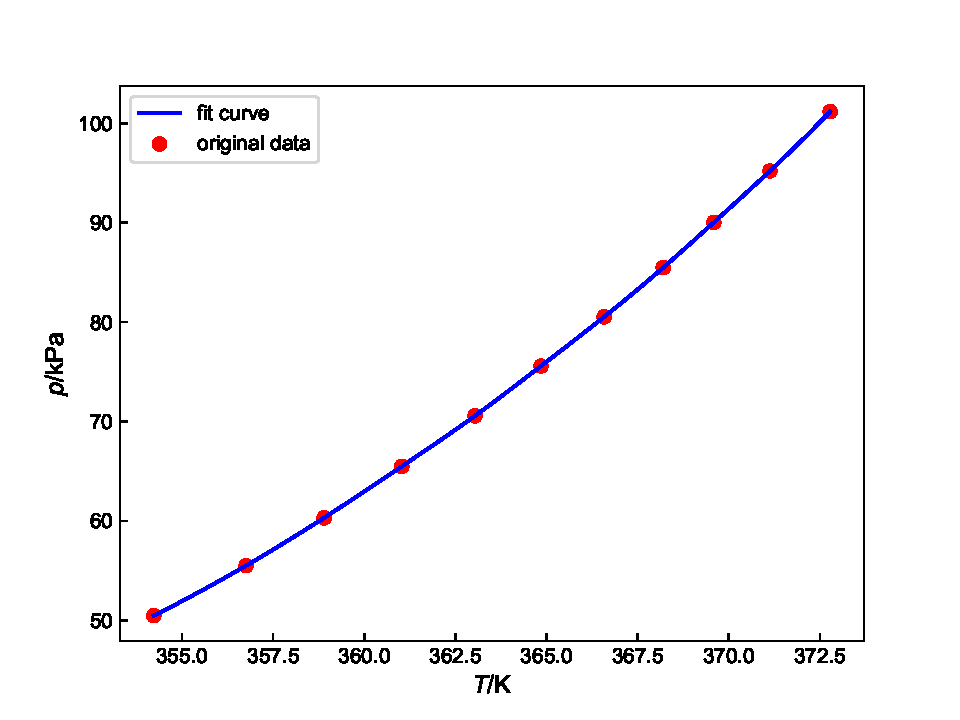
\includegraphics[width=0.6\textwidth]{water_spline.pdf}
			\bicaption{\ce{H2O}的饱和蒸汽压与温度的关系}{the relation between vapour pressure of \ce{H2O} and temperature}
			\label{P-T spline of H2O}
		\end{figure}
		采用与之前一样的方法可以得到线性回归的结果如图\ref{P-T of H2O}。
		\begin{figure}[h]
			\centering
			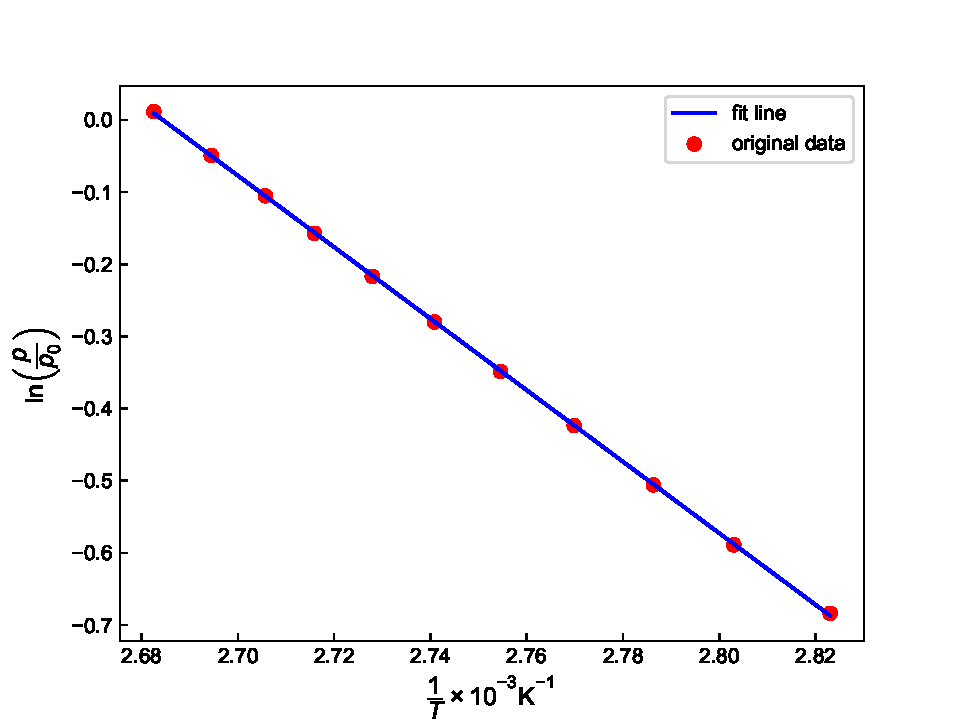
\includegraphics[width=0.6\textwidth]{water.pdf}
			\bicaption{\ce{H2O}的饱和蒸汽压与温度的关系}{the relation between vapour pressure of \ce{H2O} and temperature}
			\label{P-T of H2O}
		\end{figure}
		从图中可以看出很好的线性相关性,同时回归方程为:
		\begin{equation}
			\ln\left(\dfrac{p}{p^{\circ}}\right) = -\dfrac{-4956\pm 11}{T} + 13.30
		\end{equation}
		可以计算出\ce{H2O}的蒸发焓为$\Delta_{vap}H_{m} = 41.20\pm 0.09\,\mr{kJ/mol}$,
		带入$p = 101.3\mr{kPa}$可以计算出正常沸点为$T_b = 99.7\pm0.2\celsius$。进一步可以计算出
		正常沸点下的摩尔气化熵$\Delta_{vap}S_{m} = 110.6\pm0.2\,\mr{J/(mol\,K)}$,这与Trouton
		规则有了明显的正偏差。
 	
 		 

	\vbox{}  	
 	\section{讨论与结论}
		\subsection{实验讨论}
 		\subsubsection{本实验测得的摩尔气化焓与标准值的比较}
		通过查阅资料得知\citealp{2012CRC},\ce{CCl4}的标准摩尔蒸发焓为$32.54\mr{kJ/mol}$
		(注意这是298K下的数据),
		可以看出在本实验中测量值小于298K时的数据(本实验的温度高于298K);
		\ce{H2O}的标准摩尔蒸发焓为$44.0\mr{kJ/mol}$,而
		在沸点时的蒸发焓为$40.68/\mathrm{kJ/mol}$(差异就是来源于
		液态水有较大的热容,在Clapeyron方程中忽略掉是不好的近似),本实验测量值依然小于298K的数据。
		\par 考虑在两个温度下的蒸发焓的关系,由盖斯定律容易得到:
		\begin{equation}
			\Delta_{vap}H_{m}(T_2) = \Delta_{vap}H_{m}(T_1) + \int_{T_1}^{T_2}[C_{p,g}(T) - C_{p,l}(T)]\d T
		\end{equation}
		可以从上式看出,如果液相有着明显大于气相的热容,那么就会导致温度上升时蒸发焓明显减小,
		为此查阅相关数据\citealp{doi:10.1021/ja01235a002},得到\ce{CCl4}的恒压热容
		$C_{p,g} = 82.65\mr{J/(mol\,K)}\,\,C_{p,l} = 131.3\mr{J/(mol\,K)}$;
		得到水的恒压热容数据(100K)$C_{p,g} = 35.6\mr{J/(mol\,K)}\,\,C_{p,l} = 75.94\mr{J/(mol\,K)}$,
		可以看到液相热容均明显大于气相热容,这就解释了实验中测得的蒸发焓较298K时的值偏小。可以简单估算
		(由前面的气液两相热容差乘上实验温度与298K之差),
		由热容导致的蒸发焓的变化在$1\mr{kJ/mol}$的量级,远大于实验本身产生的误差,这应该是我们对于Clapeyron
		方程近似的过程中产生的主要误差,而忽略掉凝聚相体积(对水而言,凝聚相体积小于气相体积的千分之一)和
		理想气体近似产生的误差相对很小。

 	 	\subsubsection{本实验测得的摩尔气化熵与Trouton规则比较}
 	 	\ce{CCl4}测得的正常沸点下的气化熵为$\Delta_{vap}S_{m} = 90.0\mr\pm0.02{J/mol;\,K}$,与Trouton规则非常接近,但是
		水的气化熵$\Delta_{vap}S_{m} = 110.6\pm0.2\,\mr{J/(mol\,K)}$远高于Trouton规则,在查阅维基百科
		后了解到Trouton规则对非极性液体比较适用,对于极性液体、尤其是含有氢键的体系不适用。可能的解释是氢键
		让某一相产生了有序的结构,从而降低了熵使之偏离Trouton规则,比如说由于氢键存在水在液相会形成有序结构,
		导致液相熵减小从而产生对于Trouton规则的正偏差;而甲酸由于在气相也会以二聚物的形式存在,气相的熵比较小
		($61.8\mr{J/mol}$\citealt{formic_acid_wiki}),
		因此会对Trouton规则产生负偏差。
 	 	\subsection{实验结论}
 	 	本实验使用静态法测定不同温度下\ce{CCl4}的饱和蒸气压,使用动态法测定水在不同压力下的沸点,
		利用Clapeyron方程对结果拟合,得到\ce{CCl4}和水的摩尔气化热分别为$31.43\pm0.06\,\mr{kJ/mol}$
		和$41.20\pm0.09\,\mr{kJ/mol}$;正常沸点分别为$76.0\pm0.2\,\celsius$和
		$99.7\pm0.2\,\celsius$;摩尔气化熵分别为$90.0\pm0.02\,\mr{J/(mol\,K)}$和
		$110.6\pm0.02\,\mr{J/(mol\,K)}$,并与准确值进行了对比,解释了差异产生的原因
		。从结果可以看出,\ce{CCl4}对Trouton规则符合得较好,
		而水则与该规则偏差较大,其原因在于液态水中氢键促使了有序结构的形成,减小了液态熵。
	\section{致谢}
	感谢杨老师的悉心指导与同组各位同学的帮助!
	\vbox{}  
	\bibliographystyle{achemso}
	\bibliography{cite}



\end{document}